

\chapter{Hardware Implementation of BCH Encoder} \label{ch:BCHencImpl}

%\section{Serial Architectures}
%\section{Parallel Architecture}

\section{FEC Encoding Section}

The parallelism of the input memory of the LDPC encoding section suggests a \(p = 8\) degree of parallelism for BCH architecture. First, because LDPC input memory requires 360 bits and LDPC encoder processes the same number of bits at every clock ticks (i.e., it has 360 as degree of parallelism). Hence, \(p\) should be a divisor of 360.
Second, \(p\) should be even a divisor of each BCH block length (\(n\ped{bch}\)) associated to LDPC coding rates, provided by DVB-S2.
Furthermore, BCH serial architectures based on LFSRs are, of course, simple to implement, but generally they are very slow (i.e., they reach typically a lower throughput). Therefore, in order to best match BCH encoding speed with the frequency requirements imposed by the overall designed TX DVB-S2 section, we have chosen a degree of parallelism equal to 8.

Encoded bits, passing through an interface circuit, enter LDPC input memory on a byte basis. The interface allows each codeword coming from BCH encoder to be read in the proper order and format (recall that a systematic code is required as output). A block diagram of the overall FEC section is depicted in \figref{fig:ovrsys}.

\begin{figure} \centering
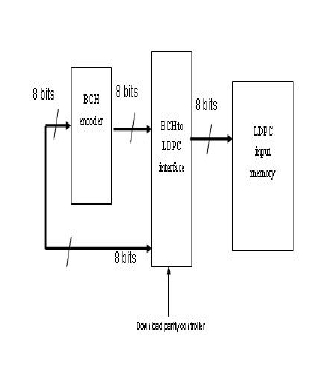
\includegraphics[width = 0.8\linewidth, height= 0.35\textheight]{FECARCH}
\caption{Block diagram of the overall FEC tx section} \label{fig:ovrsys}
\end{figure}

As we shall detail in the next section, the interface between BCH and LDPC is constituted by a simple 8 bits multiplexer together with a suited circuitry to store and download the parity bits after each computation cycle. This interface addresses properly encoded bits into LDPC input memory and it must be driven by a control logic based on clock cycles required (see \tbref{tb:clkreq}) to provide a codeword.

Another important question to raise up is certainly giving the architecture a flexible structure so as to succeed in dealing with each coding rate provided by DVB-S2 FEC. A more versatility, as we shall see, requires an additional usage of memory: as a matter of fact, some additional coefficient of matrices mentioned in the previous chapter must be stored into some LUTs (Look Up Tables).

\begin{table} \centering
\begin{tabular}{||p{2.44cm}||p{2.5cm}||p{2.53cm}||p{2.28cm}||p{2.06cm}||}
\hline
 \multicolumn{1}{|p{2.44cm}|}{\centering BCH Uncoded Block} &  \multicolumn{1}{p{2.5cm}|}{\centering BCH Coded Block \(N\ped{BCH}\)} &  \multicolumn{1}{p{2.53cm}|}{\centering Ticks to transmit informative bits} &  \multicolumn{1}{p{2.28cm}|}{\centering Parity bits download} &  \multicolumn{1}{p{2.06cm}|}{\centering Total clock cycles} \\
\hline
 \multicolumn{1}{|p{2.44cm}|}{\centering 16008} &  \multicolumn{1}{p{2.5cm}|}{\centering 16200} &  \multicolumn{1}{p{2.53cm}|}{\centering 2001} &  \multicolumn{1}{p{2.28cm}|}{\centering 24} &  \multicolumn{1}{p{2.06cm}|}{\centering 2025} \\
 \multicolumn{1}{|p{2.44cm}|}{\centering 21408} &  \multicolumn{1}{p{2.5cm}|}{\centering 21600} &  \multicolumn{1}{p{2.53cm}|}{\centering 2676} &  \multicolumn{1}{p{2.28cm}|}{\centering 24} &  \multicolumn{1}{p{2.06cm}|}{\centering 2700} \\
 \multicolumn{1}{|p{2.44cm}|}{\centering 25728} &  \multicolumn{1}{p{2.5cm}|}{\centering 25920} &  \multicolumn{1}{p{2.53cm}|}{\centering 3216} &  \multicolumn{1}{p{2.28cm}|}{\centering 24} &  \multicolumn{1}{p{2.06cm}|}{\centering 3240} \\
 \multicolumn{1}{|p{2.44cm}|}{\centering 32208} &  \multicolumn{1}{p{2.5cm}|}{\centering 32400} &  \multicolumn{1}{p{2.53cm}|}{\centering 4026} &  \multicolumn{1}{p{2.28cm}|}{\centering 24} &  \multicolumn{1}{p{2.06cm}|}{\centering 4050} \\
 \multicolumn{1}{|p{2.44cm}|}{\centering 38688} &  \multicolumn{1}{p{2.5cm}|}{\centering 38880} &  \multicolumn{1}{p{2.53cm}|}{\centering 4836} &  \multicolumn{1}{p{2.28cm}|}{\centering 24} &  \multicolumn{1}{p{2.06cm}|}{\centering 4860} \\
 \multicolumn{1}{|p{2.44cm}|}{\centering 43040} &  \multicolumn{1}{p{2.5cm}|}{\centering 43200} &  \multicolumn{1}{p{2.53cm}|}{\centering 5380} &  \multicolumn{1}{p{2.28cm}|}{\centering 20} &  \multicolumn{1}{p{2.06cm}|}{\centering 5400} \\
 \multicolumn{1}{|p{2.44cm}|}{\centering 48408} &  \multicolumn{1}{p{2.5cm}|}{\centering 48600} &  \multicolumn{1}{p{2.53cm}|}{\centering 6051} &  \multicolumn{1}{p{2.28cm}|}{\centering 24} &  \multicolumn{1}{p{2.06cm}|}{\centering 6075} \\
 \multicolumn{1}{|p{2.44cm}|}{\centering 51648} &  \multicolumn{1}{p{2.5cm}|}{\centering 51840} &  \multicolumn{1}{p{2.53cm}|}{\centering 6456} &  \multicolumn{1}{p{2.28cm}|}{\centering 24} &  \multicolumn{1}{p{2.06cm}|}{\centering 6480} \\
 \multicolumn{1}{|p{2.44cm}|}{\centering 53840} &  \multicolumn{1}{p{2.5cm}|}{\centering 54000} &  \multicolumn{1}{p{2.53cm}|}{\centering 6730} &  \multicolumn{1}{p{2.28cm}|}{\centering 20} &  \multicolumn{1}{p{2.06cm}|}{\centering 6750} \\
 \multicolumn{1}{|p{2.44cm}|}{\centering 57472} &  \multicolumn{1}{p{2.5cm}|}{\centering 57600} &  \multicolumn{1}{p{2.53cm}|}{\centering 7184} &  \multicolumn{1}{p{2.28cm}|}{\centering 16} &  \multicolumn{1}{p{2.06cm}|}{\centering 7200} \\
 \multicolumn{1}{|p{2.44cm}|}{\centering 58192} &  \multicolumn{1}{p{2.5cm}|}{\centering 58320} &  \multicolumn{1}{p{2.53cm}|}{\centering 7274} &  \multicolumn{1}{p{2.28cm}|}{\centering 16} &  \multicolumn{1}{p{2.06cm}|}{\centering 7290} \\
\hline
\end{tabular}
\caption{Clock cycles required to provide each codeword for each operating mode of DVB-S2} \label{tb:clkreq}
\end{table}

\section{Encoder Description}

A block diagram of BCH encoder architecture is shown in \figref{fig:HWarch}. A brief description on its functioning is given below.
\begin{itemize}
\item All the informative \(k\ped{bch}\) bits enter in parallel (\(p\) bits, i.e., 8 at once), from MSB to LSB, all 192 combinatorial blocks, which perform logic function indicated by \(\vet B_p\) matrix. In other words, each block carries out a row by columns product (over \(GF(2)\)) between the \(i\)-th row of \(\vet B_p\) the \(p\) inputs. Since operations are in GF(2), sums are implementable by XOR gates, multiplications by AND gates. \figref{fig:COMBin} gives a schematic illustration of each combinatorial networks processing \(p\) inputs.
\item  Each flip-flop labelled by \(x_i\) represents a single bit of state vector \(\vet x\) of the system and after exactly \(\frac{k\ped{bch}}{p}\) clock ticks it contains the result of division algorithm.
\item  Combinatorial networks toward the BCH-to-LDPC interface (i.e, on the output side) perform the feedback: each XOR gate is fed by the last \(p\) bits of register state \(\vet x\) (from \(x_{184}\) to \(x_{191}\)) passing through output-combinatorial network described by the two sub-matrices \(\vet C_1\) and \(\vet C_2\) (see \secref{sec:Regularity}). More in details, expression \eqref{eq:Apreg} in \secref{sec:Regularity}, showing an high regularity of \(\vet A^p\), allows to split computation of the first term in \eqref{eq:SEmatr} (i.e, \(\vet A^p \vet x \left[ (i-1)p \right]\)) in two contributes
    \begin{enumerate}
    \item row by column products involving last \(p\) bits of \(\vet x\) and therefore last \(p\) columns of matrix \(\vet A^p\). In other words, the combinatorial networks near to BCH-LDPC interface perform the following product
        \begin{equation} \label{eq:prodotto}
        \left(
        \begin{array}{c}
        \vet C_1 \\
        \vet C_2
        \end{array}
        \right)
        \left(
        \begin{array}{c}
        x_{184}(i) \\
        \vdots \\
        x_{191}(i)
        \end{array}
        \right)
        \end{equation}
     \item 	row by column product involving (starting from bit \(x_8\) of vector \(\vet x\) which correspond to row 9 of matrix \(\vet A^p\)) first \(n-k-p\) bits of vector \(\vet x\) is realized by sum modulo 2 (i.e., XOR gates) nodes on the right of the combinatorial networks. \figref{fig:COMBout} gives a schematic representation of this combinatorial networks together with modulo 2 sum nodes.
     \end{enumerate}
\item Logic functions relevant to sub-matrix \(\vet I\) of \(\vet A^p\) are implemented by XOR gates at the output of combinatorial networks connected to the last \(p\) bits of the state vector.
\item At the end of each computation cycle, the encoder register must be reset.
\end{itemize}

Due to intrinsic simplicity of matrices \(\vet A^p\) and \(\vet B_p\) (they are only composed by zeroes and ones), the two combinatorial networks can be implemented in a very simple way by programmable XOR gates with eight inputs.
More in detail, each coefficient of the above two matrices says which wires have to be connected to each combinatorial network (XOR).


\tikzstyle{8XOR}=[draw, minimum height=9cm, text centered,					
                  inner sep= 0pt, text width= 4em, minimum width= 3cm]

\begin{figure}
\begin{signalflow}[]
\node[input] (i1) {\(x_{184}\)};
\node[input] (i2) [below from=i1] {\(x_{185}\)};
\node[input] (i3) [below from=i2] {\(x_{186}\)};
\node[input] (i4) [below from=i3] {\(x_{187}\)};
\node[input] (i5) [below from=i4] {\(x_{188}\)};
\node[input] (i6) [below from=i5] {\(x_{189}\)};
\node[input] (i7) [below from=i6] {\(x_{190}\)};
\node[input] (i8) [below from=i7] {\(x_{191}\)};
\node[multiplier] (m1) [right from= i1,label=above:\(a_{j\virgola 184}\)] {};
\node[multiplier] (m2) [right from= i2,label=above:\(a_{j\virgola 185}\)] {};
\node[multiplier] (m3) [right from= i3,label=above:\(a_{j\virgola 186}\)] {};
\node[multiplier] (m4) [right from= i4,label=above:\(a_{j\virgola 187}\)] {};
\node[multiplier] (m5) [right from= i5,label=above:\(a_{j\virgola 188}\)] {};
\node[multiplier] (m6) [right from= i6,label=above:\(a_{j\virgola 189}\)] {};
\node[multiplier] (m7) [right from= i7,label=above:\(a_{j\virgola 190}\)] {};
\node[multiplier] (m8) [right from= i8,label=above:\(a_{j\virgola 191}\)] {};
\node[8XOR] (8XOR) [right from=m4] {\Huge XOR};
\node[coordinate] (c1) [right from=8XOR] {};
\node[adder] (a1) [right from=c1] {};
\node[input] (x) [above from=a1, label=above:{\(x_{j-8}(i)\) for \(j \geq 8\)}] {};
\node[output] (out) [right from=a1, label=right:{\(y_j(i)\)}] {};
% signal path
\path[r>] (i1)--(m1);
\path[r>] (i2)--(m2);
\path[r>] (i3)--(m3);
\path[r>] (i4)--(m4);
\path[r>] (i5)--(m5);
\path[r>] (i6)--(m6);
\path[r>] (i7)--(m7);
\path[r>] (i8)--(m8);
\path[r>] (m1) -- +(1,0);
\path[r>] (m2) -- +(1,0);
\path[r>] (m3) -- +(1,0);
\path[r>] (m4) -- +(1,0);
\path[r>] (m5) -- +(1,0);
\path[r>] (m6) -- +(1,0);
\path[r>] (m7) -- +(1,0);
\path[r>] (m8) -- +(1,0);
\path[r] (8XOR) -- (c1);
\path[r>] (x)--(a1);
\path[r>] (c1)--(a1);
\path[r>] (a1)--(out);
\end{signalflow}
\caption{Block scheme of the combinatorial networks acting on the last \(p\) bits of \(\vet x\). \(a_{j \virgola l}\) is the coefficient at \(j\)-th row and \(l\)-th column of \(\vet A^8\) matrix }\label{fig:COMBout}
\end{figure}

\begin{figure}
\begin{signalflow}[]
\node[input] (i1) {\(u(ip-1)\)};
\node[input] (i2) [below from=i1] {\(u(ip-2)\)};
\node[input] (i3) [below from=i2] {\(u(ip-3)\)};
\node[input] (i4) [below from=i3] {\(u(ip-4)\)};
\node[input] (i5) [below from=i4] {\(u(ip-5)\)};
\node[input] (i6) [below from=i5] {\(u(ip-6)\)};
\node[input] (i7) [below from=i6] {\(u(ip-7)\)};
\node[input] (i8) [below from=i7] {\(u[p(i-1)]\)};
\node[multiplier] (m1) [right from= i1,label=above:\(b_{j\virgola 0}\)] {};
\node[multiplier] (m2) [right from= i2,label=above:\(b_{j\virgola 1}\)] {};
\node[multiplier] (m3) [right from= i3,label=above:\(b_{j\virgola 2}\)] {};
\node[multiplier] (m4) [right from= i4,label=above:\(b_{j\virgola 3}\)] {};
\node[multiplier] (m5) [right from= i5,label=above:\(b_{j\virgola 4}\)] {};
\node[multiplier] (m6) [right from= i6,label=above:\(b_{j\virgola 5}\)] {};
\node[multiplier] (m7) [right from= i7,label=above:\(b_{j\virgola 6}\)] {};
\node[multiplier] (m8) [right from= i8,label=above:\(b_{j\virgola 7}\)] {};
\node[8XOR] (8XOR) [right from=m4] {\Huge XOR};
\node[coordinate] (c1) [right from=8XOR] {};
\node[adder] (a1) [right from=c1] {};
\node[input] (x) [above from=a1, label=above:{\(y_{j}(i)\)}] {};
\node[output] (out) [right from=a1, label=right:{\(x_j(i+1)\)}] {};
% signal path
\path[r>] (i1)--(m1);
\path[r>] (i2)--(m2);
\path[r>] (i3)--(m3);
\path[r>] (i4)--(m4);
\path[r>] (i5)--(m5);
\path[r>] (i6)--(m6);
\path[r>] (i7)--(m7);
\path[r>] (i8)--(m8);
\path[r>] (m1) -- +(1,0);
\path[r>] (m2) -- +(1,0);
\path[r>] (m3) -- +(1,0);
\path[r>] (m4) -- +(1,0);
\path[r>] (m5) -- +(1,0);
\path[r>] (m6) -- +(1,0);
\path[r>] (m7) -- +(1,0);
\path[r>] (m8) -- +(1,0);
\path[r] (8XOR) -- (c1);
\path[r>] (x)--(a1);
\path[r>] (c1)--(a1);
\path[r>] (a1)--(out);
\end{signalflow}
\caption{Block scheme representing the combinatorial networks acting on the \(p\) bit of input. \(b_{j \virgola l}\) is the coefficient at \(j\)-th row and \(l\)-th column of the \(\vet B_8\) matrix} \label{fig:COMBin}
\end{figure} 

\section{Dealing with Each Error Protection}

Architecture we have shown as far can only address the greater \(t\) error protection modalities. However, DVB-S2 has been designed to operate in ACM (Adaptive Coding and Modulation) mode, so that a flexible architecture, capable of changing his behavior on a frame basis, would be more desirable.

From our analysis of the two matrices, we have reach the conclusion that they are very regular and, even changing the polynomial generator of the code, this interesting property still holds. The degree of parallelism \(p\), once set by design, cannot vary. Henceforth all our considerations will be constrained to a specific degree of parallelism, \(p=8\), even though the method we are going to show is general at all.

BCH of DVB-S2 provides three protection level \(t = 8\virgola 10 \virgola 12\) associated to the following different generators
\begin{align}
g\ped{t_{12}}(x) & = g_1(x)g_2(x)\ldots g_{12}(x) \label{eq:BCHt12}\\
g\ped{t_{10}}(x) & = g_1(x)g_2(x)\ldots g_{10}(x) \label{eq:BCHt10}\\
g\ped{t_8}(x) & = g_1(x)g_2(x)\ldots g_{8}(x) \label{eq:BCHt8}
\end{align}
where the above polynomials are in \tbref{tb:BCHpoly}.
According to the decrease of the degree of polynomial generator, also the number \(r\) of redundancy bits decreases and thus the number of FFs illustrated in \figref{fig:HWarch} would be oversized. This implies that, \(\vet x\) being changed, size of matrices \(\vet A^8\) and \(\vet B_8\) has to change. In \secref{sec:Regularity} we have shown that, for a reasonable level of parallelism, matrix \(\vet A^p\) shows some regularity. In practice, its structure shown in \eqref{eq:Apreg} does not change from \(t_8\) to \(t_{12}\), although its coefficients are, of course, subject to variations. Same consideration can be made upon \(\vet B_p\) matrix, which however shows no regularity property for this kind of architecture.

\figref{fig:COMBin} and \figref{fig:COMBout} clearly show that these kind of combinatorial network are programmable by means of their coefficients, determining which wire has to be connected to the 8-inputs XOR gate and which not. Imposing, for example, that all of these coefficients are forced to zero, we would get the result of having inhibited the \(j\)-th combinatorial network. This is exactly what we can do to deal with all the protection level \(t\).

In particular, either \(\vet A^8\) or \(\vet B_8\) can be embedded into the their largest matrices of size, respectively, \(192 \times 192\) and \(192 \times 8\) in this way:
\begin{description}
\item[Medium Protection Level](\(t=10\)) Matrices \((\vet A^8)\ped{o}\) and \((\vet B_8)\ped{o}\) oversized (they should be \(160 \times 160\) and \(160 \times 8\) respectively) turn out to be as follows
    \begin{align}
    (\vet A^8)\ped{o} &=
    \left(
    \begin{array}{cc}
    \vet 0 & \vet 0 \\
    \vet 0 & (\vet A^8)\ped{t_{10}}
    \end{array}
    \right) &
    (\vet B_8)\ped{o} &=
    \left(
    \begin{array}{c}
    \vet 0 \\
    (\vet B_8)\ped{t_{10}}
    \end{array}
    \right)
    \end{align} \label{eq:embedding}
    This corresponds to inhibit the first 32 couples of combinatorial networks since their coefficients are all nulls. Thus, all the first 32 FFs (from \(x_0\) to \(x_{31}\)) of the BCH encoder will contain always zeroes.
\item[Low Protection Level](\(t=8\)) The oversized matrices are build in the same manner and now the first 64 couples of combinatorial networks are inhibited since their coefficients are all nulls.
\end{description}

\begin{figure} \centering
%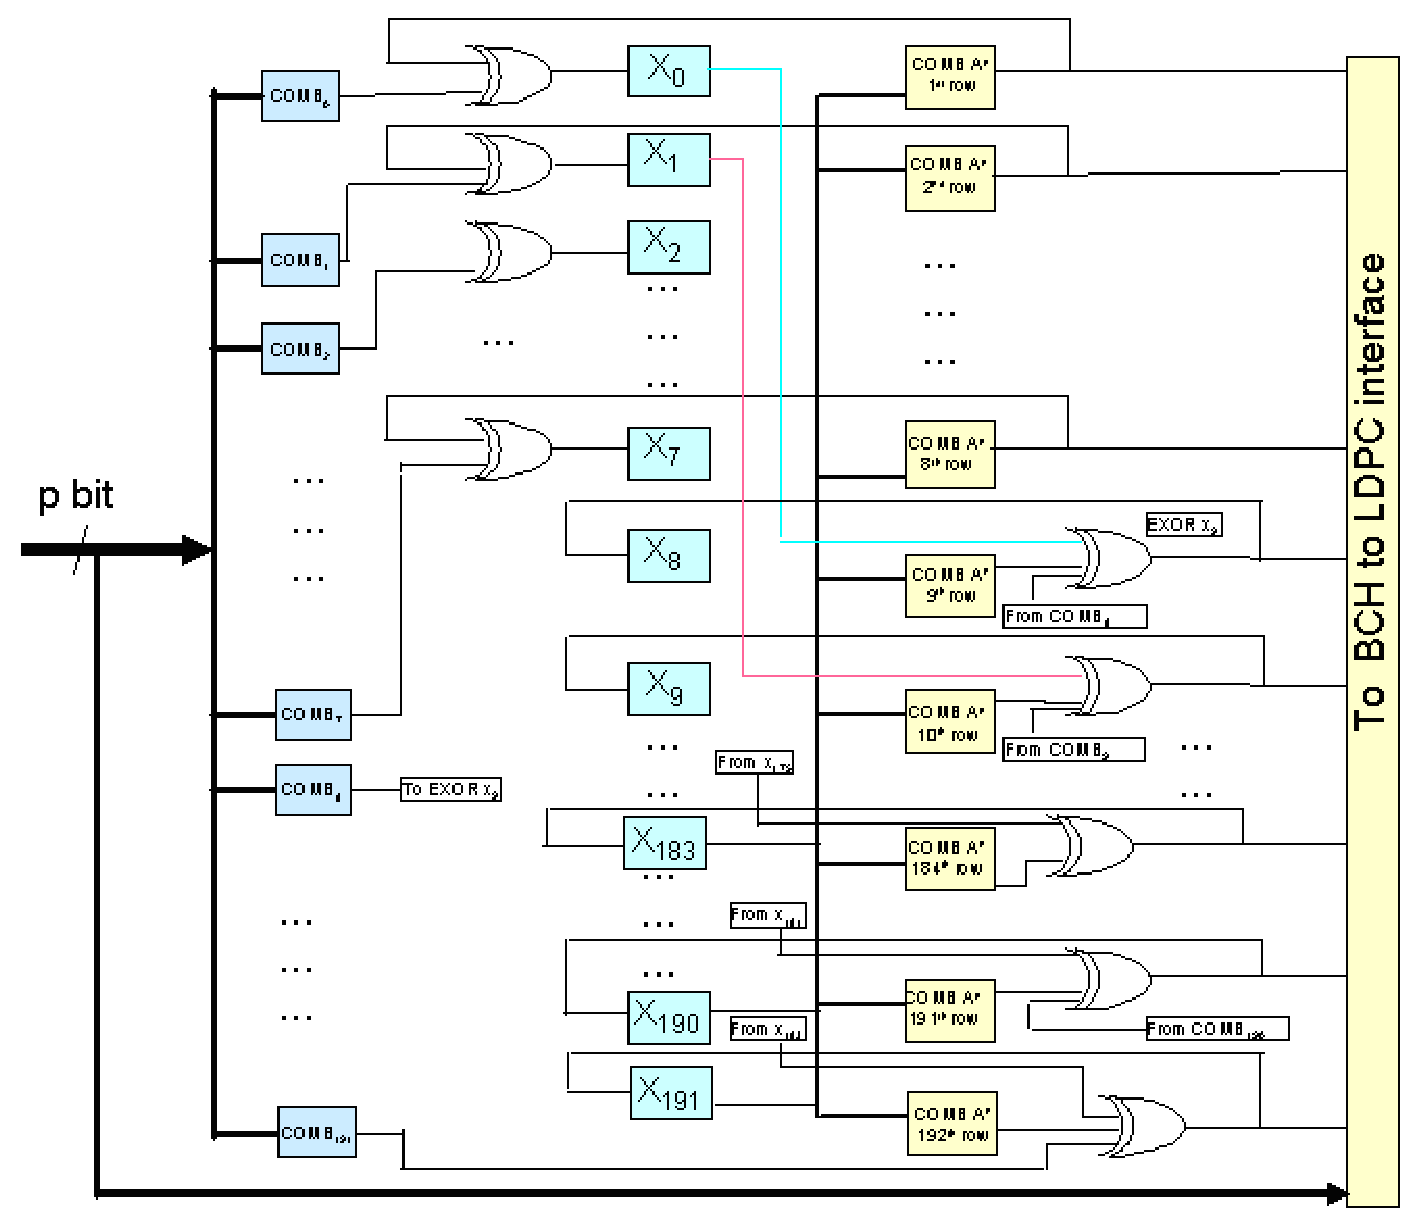
\includegraphics[width = 0.8\linewidth, height= 0.8\textheight]{encblock}
\tikzstyle{BUS}
 = [line width=2pt,
      >= real tip,
      draw]
\tikzstyle{phan}
  = [minimum size=\delaysize]
\begin{signalflow}[node distance=1cm]
\node[coordinate] (c1)  {};
%
%\node[coordinate] (c183) [below from=c182] {};
%\node[coordinate] (c184) [below from=c183] {};
%\node[coordinate] (c186) [below from=c184] {};
%\node[coordinate] (c191) [below from=c186] {};
%% Input Combinatorials
\node[delay] (a1)  [right from=c1] {\(\vet b_1 \vet u\)};
\node[delay] (a2) [below from=a1] {\(\vet b_2 \vet u\)};
\node[phan] (a3) [below from=a2] {\(\vdots\)};
\node[delay] (a8) [below from=a3] {\(\vet b_8 \vet u\)};
\node[delay] (a9) [below from=a8] {\(\vet b_9 \vet u\)};
\node[phan]  (phh) [below from=a9] {\(\vdots\)};
\node[delay] (a183) [below from=phh] {\(\vet b_{184} \vet u\)};
\node[delay] (a184) [below from=a183] {\(\vet b_{185} \vet u\)};
\node[phan] (a186) [below from=a184] {\(\vdots\)};
\node[delay] (a191) [below from=a186] {\(\vet b_{192} \vet u\)};
%% Some coordinates
\node[coordinate] (c2) [left from=a2] {};
\node[coordinate] (c3) [left from=a8] {};
\node[coordinate] (c4) [left from=a9] {};
\node[coordinate] (c9) [below from=c4, below=2.37cm] {};
\node[coordinate] (c182) [below from=c9,below=.63cm] {};
\node[coordinate] (c183) [left from=a191, right=.14cm] {};

\node[coordinate] (input) [left from=c9] {};
%% First XORs stage
\node[adder]  (x1) [right from=a1, left=0cm] {};
\node[adder]  (x2) [right from=a2,left=0cm] {};
\node[adder]  (x8) [right from=a8,left=0cm] {};
\node[adder]  (x9) [right from=a9,left=0cm] {};
\node[adder]  (x183) [right from=a183,left=0cm] {};
\node[adder]  (x184) [right from=a184,left=0cm] {};
\node[adder]  (x191) [right from=a191,left=0cm] {};
%% Feedbacks
\node[input]  (i1) at (x1) [above= .65cm,label=right:{\(y_0\)}] {};
\node[input]  (i2) at (x2) [above= .65cm,label=right:{\(y_1\)}] {};
\node[input]  (i8) at (x8) [above= .65cm,label=right:{\(y_7\)}] {};
\node[input]  (i9) at (x9) [above= .65cm,label=right:{\(y_8\)}] {};
\node[input]  (i183) at (x183) [above= .65cm,label=right:{\(y_{183}\)}] {};
\node[input]  (i184) at (x184) [above= .65cm,label=right:{\(y_{184}\)}] {};
\node[input]  (i191) at (x191) [above= .65cm,label=right:{\(y_{191}\)}] {};
%% Register of state
\node[delay]  (s1) [right from=x1] {\(x_0\)};
\node[delay]  (s2) [right from=x2] {\(x_1\)};
\node[delay]  (s8) [right from=x8] {\(x_7\)};
\node[delay]  (s9) [right from=x9] {\(x_8\)};
\node[phan]   (ph) [below from=s9] {\(\vdots\)};
\node[delay]  (s183) [below from=ph] {\(x_{183}\)};
\node[delay]  (s184) [below from=s183] {\(x_{184}\)};
\node[phan] (sp) [below from=s184] {\(\vdots\)};
\node[delay]  (s191) [below from=sp] {\(x_{191}\)};

%% Outputs
\node[output] (so1) [right from=s1] {};
\node[output] (so2) [right from=s2] {};
\node[output] (so8) [right from=s8] {};
\node[output] (so9) [right from=s9] {};
\node[output] (so183) [right from=s183, left=0cm] {};

%% Bus on the right side
%\node[coordinate] (cc184) [right from=s191] {};
%\node[coordinate] (cc9) [above from=cc184] {};
%\node[coordinate] (cc8) [above from=cc9] {};
%\node[coordinate] (cc2) [above from=cc8] {};
%\node[coordinate] (cc7) [above from=cc8] {};
%\node[coordinate] (cc6) [above from=cc7] {};
%\node[coordinate] (cc3) [above from=cc6] {};
%\node[coordinate] (cc2) [above from=cc3] {};
%\node[coordinate] (cc1) [above from=cc2] {};
\node[coordinate] (cc191) [right from=s191, right=1cm] {};
\node[coordinate] (cc186) [right from=s184, right=1cm] {};
\node[coordinate] (cc183) [right from=s183, right=1cm] {};
\node[coordinate] (cc9)   [right from=s9, right=1.15cm] {};
\node[coordinate] (cc8)  [right from=s8, right=1.15cm] {};
\node[coordinate] (cc2) [right from=s2, right=1.15cm] {};
\node[coordinate] (cc1) [right from=s1, right=1.15cm] {};

%% Cominatorial networks on the right side
\node[delay] (b1) [right from=cc1] {};
\node[delay] (b2) [right from=cc2] {};
\node[phan] (b3)  [below from=b2] {\(\vdots\)};
\node[delay] (b4) [right from=cc8] {};
\node[delay] (b5) [right from=cc9] {};
\node[delay] (b6) [right from=cc183] {};
\node[delay] (b7) [right from=cc186] {};
\node[delay] (b8) [right from=cc191] {};

%% At the output of the above combinatorial
\node[output] (n1) [right from=b1, label=right:{\(y_0\)}, right=1cm] {};
\node[output] (n2) [right from=b2, label=right:{\(y_1\)}, right=1cm] {};
\node[output] (n3) [right from=b4, label=right:{\(y_7\)}, right=1cm] {};
\node[adder]  (n4) [right from=b5] {};
\node[output] (n4b) [right from=n4, label=right:{\(y_8\)}]  {};
\node[adder]  (n5) [right from=b6] {};
\node[output] (n5b) [right from=n5, label=right:{\(y_{183}\)}]  {};
\node[adder]  (n6) [right from=b7] {};
\node[output] (n6b) [right from=n6, label=right:{\(y_{184}\)}]  {};
\node[adder]  (n7) [right from=b8] {};
\node[output] (n7b) [right from=n7, label=right:{\(y_{191}\)}]  {};

\node[input]  (ii4) at (n4) [above= .65cm,label=right:{\(x_0\)}] {};
\node[input]  (ii5) at (n5) [above= .65cm,label=right:{\(x_{175}\)}] {};
\node[input]  (ii6) at (n6) [above= .65cm,label=right:{\(x_{176}\)}] {};
\node[input]  (ii7) at (n7) [above= .65cm,label=right:{\(x_{183}\)}] {};
%\node[input]  (i183) at (x183) [above= .65cm,label=right:{\(y_{183}\)}] {};
%\node[input]  (i184) at (x184) [above= .65cm,label=right:{\(y_{184}\)}] {};
%\node[input]  (i191) at (x191) [above= .65cm,label=right:{\(y_{191}\)}] {};

%%% BUS WIRES
\path[BUS] (c1)--(c2)--(c3)--(c4)--(c9)--(c182)--(c183)
            (c1)--(a1)
            (c2)--(a2)
            (c3)--(a8)
            (c4)--(a9)
            (c9)--(a183)
            (c183)--(a191)
            (c182)--(a184);
\path[BUS]  (cc191)--(cc183)--(cc9)--(cc8)--(cc2)--(cc1);


%%% COMB1 to adder connections
\path[r>]   (a1)--(x1);
\path[r>]   (a2)--(x2);
\path[r>]   (a8)--(x8);
\path[r>]   (a9)--(x9);
\path[r>]   (a183)--(x183);
\path[r>]   (a184)--(x184);
\path[r>]   (a191)--(x191);

%%%% State register outputs
\path[r>]   (s1)--(so1);
\path[r>]   (s2)--(so2);
\path[r>]   (s8)--(so8);
\path[r>]   (s9)--(so9);
\path[r>]   (s183)--(so183);

%%% First adders stage to state ragister connections
\path[r>]   (x1)--(s1);
\path[r>]   (x2)--(s2);
\path[r>]   (x8)--(s8);
\path[r>]   (x9)--(s9);
\path[r>]   (x183)--(s183);
\path[r>]   (x184)--(s184);
\path[r>]   (x191)--(s191);

%% Feedback connections to the first adders stage
\path[r>]   (i1)--(x1);
\path[r>]   (i2)--(x2);
\path[r>]   (i8)--(x8);
\path[r>]   (i9)--(x9);
\path[r>]   (i183)--(x183);
\path[r>]   (i184)--(x184);
\path[r>]   (i191)--(x191);

%% Feedforward connection to the last adders stage
\path[r>]   (ii4)--(n4);
\path[r>]   (ii5)--(n5);
\path[r>]   (ii6)--(n6);
\path[r>]   (ii7)--(n7);

%% Last 8 FFs of X to BUS
\path[r]  (s184)--(cc186)
          (s191)--(cc191);

%%% COMB2 to out/adders connections
\path[r>]  (b1)--(n1);
\path[r>]  (b2)--(n2);
\path[r>]  (b4)--(n3);
\path[r>]  (b5)--(n4);
\path[r>]  (b6)--(n5);
\path[r>]  (b7)--(n6);
\path[r>]  (b8)--(n7);

%%% Last adders to output
\path[r>]  (n4)--(n4b);
\path[r>]  (n5)--(n5b);
\path[r>]  (n6)--(n6b);
\path[r>]  (n7)--(n7b);

%%% Right Hand BUSES
\path[BUS] (cc1)--(b1)
           (cc2)--(b2)
           (cc8)--(b4)
           (cc9)--(b5)
           (cc183)--(b6)
           (cc186)--(b7)
           (cc191)--(b8);
\end{signalflow} 
\caption{Architecture oriented to digital hardware implementation. Each combinatorial network on the left-hand side implements a row by column product of \(\vet B_8 \vet u\). Each row of matrix \(\vet B_8\) is indicated as \(\vet b_j\) with \(0\leq j<192\). Each combinatorial network on the right-hand side implements a row by column sub-product in \eqref{eq:prodotto}. The 8 bit bus on the input side carries message bits to be encoded.} \label{fig:HWarch}
\end{figure}


\section{Interface and Parity Bits Extraction}

The interface between BCH and LDPC encoder can be implemented as illustrated in \figref{fig:Interface}. The parity bits, once computed (at \(n\ped{bch}\) clock tick), can be saved (in a single clock cycle) in a shift register architecture, which has been called in \figref{fig:Interface} 192 (or rather, up to 192) to 8 bit converter. In fact, its task is formatting data in the DVB-S2 format. Furthermore, this kind of architecture allows to write all the parity bits extracted from BCH encoder (in a single clock tick) into LDPC input memory with a degree of parallelism equal to 8\footnote{Note also that \(p=8\) is not only a divisor for 360, but also for 192(\(t=12\)), 160(\(t=10\)) and 128(\(t=8\))}.

Further detailing, the converter is composed by 8 shift register blocks with size equal to 24 bits. In a preliminary fase all the parity bits computed by the BCH encoder are stored in these blocks following the labelling indicated in \figref{fig:Download} (to succeed in storing these bits, MUXs between each flip flop can be used). Afterward, the converter works as a shift register, thus allowing to download data eight at once, i.e., with a degree of parallelism equal to 8.

To summarize, let us see, in order for each iteration, the operations carried out by this specific interface:

\begin{enumerate}
\item Once the parity bits have been computed, they are stored in another shift register according to the bit-to-bit mapping illustrated in \figref{fig:Download}. MUXs between a FF and its neighbor allow to store bits all at once (in parallel) as they are switched on wires carrying results of encoding (these wires may be directly connected to the BCH encoder register).
\item As MUXs are switched on wires interconnecting FFs each other, all the bits previously stored, shifting along FFs, are carried by some 'strategic' wires on the 8 bits bus, which conveys parity bits toward the output multiplexer.
    Practically, the register is working as a shift register.
\item The output multiplexer has two inputs buses connected to: informative bits and redundancy bits. MUX should be driven by a proper control logic on the operating mode basis.
\end{enumerate}



\begin{figure} \centering
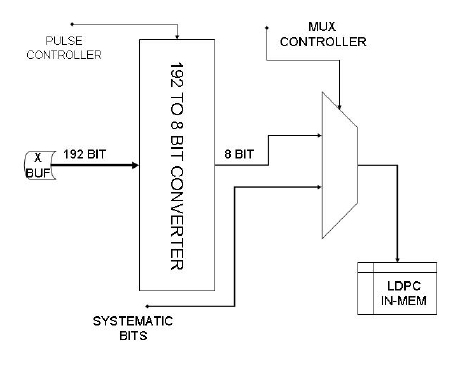
\includegraphics[scale=0.8]{Interface}
\caption{Interface architecture. Parity bits are loaded into the 192 to 8 bits converter.} \label{fig:Interface}
\end{figure}


\begin{figure} \centering
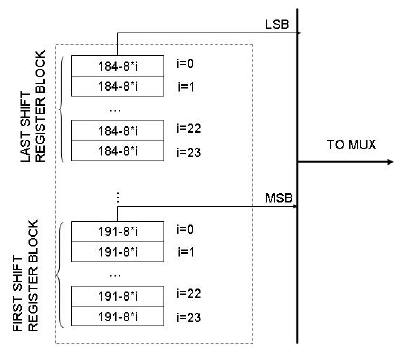
\includegraphics[scale=1]{download}
\caption{192 to 8 bits converter architecture. Values into each FF represent the index mapping between the BCH encoder register and the interface register, used to extract and format data.} \label{fig:Download}
\end{figure}


\section{Frequency and Memory Requirements}

Taking into account LDPC outer encoder frequency requirements and imposing a data rate equal to \(1 \unit{Gbps}\), in the worst case, that is, when \(t=8\) and LDPC code rate is equal to \(9/10\), we obtain the maximum frequency requirement so as to guarantee this challenging performance:
\begin{equation}
(f\ped{clk})\ped{MAX}= \frac{frame}{s}\cdot 7290 = 125 \unit{MHz}
\end{equation}
Concerning to memory requirement either, the architecture proposed takes six (two per each level of BCH protection parameter \(t\)) LUTs to store coefficients used by the combinatorial networks. As a matter of fact, storing of the \(\vet C_1\) and \(\vet C_2\) sub-matrices (recall that they represent two sub-blocks, whose aggregated size is \(192 \times 8\), of the \(\vet A^8\) matrix) coefficients as well matrix \(\vet B_8\), whose size is \(192 \times 8\), coefficients is required. To provide an encoder capable of dealing with each \(t\)-error protection level, those matrices have to be saved in LUTs for each \(t\).
The size of each LUT is equal to \(192 \unit{Bytes}\) and thus the BCH encoder, apart from additional memory required by the BCH-LDPC interface and the encoder state register, requires an amount of memory equal to
\begin{equation}
 2\cdot3\cdot192\unit{B} = 1,125\unit{KiB}.
\end{equation}

